\documentclass[UTF8]{ctexart}
\usepackage[paperwidth=9cm,paperheight=22cm,margin=6mm]{geometry}
\usepackage{graphicx}
\pagestyle{empty}
\begin{document}
\begin{center}
\vbox{\centering
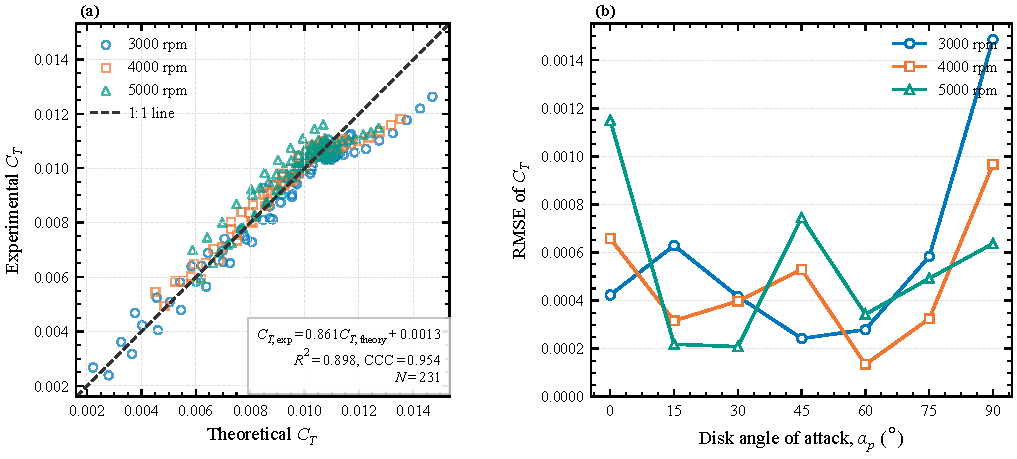
\includegraphics[width=7.5cm]{Image/fig9_rotor_model_diagnostics.pdf}\\[1mm]
{\small 图7\quad 升力系数一致性与攻角分区相对误差分布
\\ Fig.\,7 \quad Thrust coefficient agreement and relative-error distributions by disk angle of attack}\\[1mm]
\parbox{0.98\columnwidth}{\scriptsize 注：(a)参考线为1:1及相对实测值的$\pm10\%$、$\pm5\%$误差边界。(b)有符号相对误差以实测$C_T$为分母，正值表示模型低估，负值表示模型高估。每个攻角合并三个转速档位的33个不同工况；箱体为第一至第三四分位数，横线为中位数，须线延伸至1.5倍四分位距内的最远观测值，叠加显示全部工况。箱体表示工况间分布，不表示均值置信区间或33次重复试验。}
}
\end{center}
\end{document}
